\chapter{Diseño e implementación}
\label{chap:desarrollo}

Este capítulo describe el diseño y la implementación del sistema. Primero presenta la arquitectura general y sitúa los componentes que reciben los hilos de discusión, ejecutan el análisis y conservan los resultados. Después explica el modelo de facilitación, las entradas y salidas, y la secuencia interna de decisiones. Las últimas secciones describen la estrategia de contexto, el panel utilizado para ejecutar e inspeccionar los análisis y los entornos de despliegue.

\section{Arquitectura del sistema}
\label{sec:arquitectura-sistema}

La arquitectura distingue las fuentes de hilos de discusión, el servicio que realiza el análisis, el panel, los proveedores de modelos y los mecanismos utilizados para conservar e inspeccionar los resultados.

\subsection{Visión general}

El sistema se organiza alrededor del servicio de facilitación, que recibe un hilo de discusión mediante un formato común y devuelve las decisiones tomadas durante el análisis. Cuando corresponde intervenir, el resultado también incluye una respuesta candidata.

El servicio ofrece una API de Python para las llamadas directas y una API REST para los clientes remotos. De este modo, los scripts experimentales utilizan la API de Python, mientras que el panel se comunica con el servicio mediante la API REST. Además, el servicio utiliza los proveedores de modelos configurados durante el análisis y conserva los resultados y los registros técnicos para su posterior inspección.

La tabla siguiente resume los componentes principales. Las secciones posteriores explican sus contratos, su funcionamiento interno y las implementaciones empleadas durante los experimentos.

\subsection{Componentes principales}

\begin{table}[htbp]
\centering
\small
\renewcommand{\arraystretch}{1.12}
\begin{tabularx}{\textwidth}{@{}Z{3.5cm}Y@{}}
\toprule
\textbf{Componente} & \textbf{Función} \\
\midrule
Fuentes de hilos de discusión & Proporcionan las discusiones mediante el formato común de entrada. \\
Servicio de facilitación & Analiza la discusión y genera una respuesta candidata cuando corresponde. Expone una API de Python y una API REST. \\
Panel & Permite iniciar los análisis e inspeccionar sus resultados mediante la API REST. \\
Proveedores de modelos & Proporcionan los modelos utilizados por el servicio. \\
Almacenamiento y registro técnico & Conservan los resultados y la información necesaria para revisar las ejecuciones. \\
\bottomrule
\end{tabularx}
\caption{Componentes principales del sistema y su función.}
\label{tab:componentes-principales}
\end{table}

\subsection{Estructura de la implementación}

Las decisiones arquitectónicas se registraron durante el desarrollo mediante registros de decisiones de arquitectura (\textit{Architecture Decision Records}, ADRs). Esta sección describe las decisiones necesarias para entender la implementación, mientras que los ADRs conservan su razonamiento técnico y las alternativas consideradas.

El código, la integración con Open edX, los scripts, la documentación y la infraestructura se versionan en un repositorio único. Esta organización permite mantener juntos los componentes utilizados para desarrollar y evaluar el sistema. El servicio de Python se encuentra en \texttt{discussion\_moderation}, el panel en \texttt{dashboard}, la integración con Open edX en \texttt{integrations} y la automatización auxiliar en \texttt{scripts}. La estructura principal, obtenida con \texttt{tree} y reducida para omitir directorios generados y detalles internos, es la siguiente:

\begin{samepage}
\begin{small}
\begin{verbatim}
.
|-- dashboard/                 # Frontend React
|-- discussion_moderation/     # Servicio Python
|   |-- agents/
|   |-- api/
|   |-- evals/
|   |-- graph/
|   |-- rest_api/
|   `-- tools/
|-- docs/
|   |-- decisions/
|   |-- deployment/
|   |-- experiments/
|   |-- literature/
|   |-- thesis/
|   `-- threads/
|-- integrations/
|   `-- openedx/
`-- scripts/
\end{verbatim}
\end{small}
\end{samepage}

Los resultados de cada ejecución se guardan en el sistema de archivos o en S3. Un manifiesto organiza los casos por modelo e hilo de discusión y conserva las decisiones intermedias, la respuesta cuando existe, la duración, los errores y los mensajes necesarios para inspeccionar la ejecución.

\section{Modelo de facilitación}
\label{sec:modelo-facilitacion}

El modelo de facilitación describe las decisiones que realiza el servicio al analizar un hilo de discusión. El proceso se divide en tres etapas:

\begin{enumerate}
  \item \textbf{Analizar la discusión}: se clasifica el estado del hilo de discusión y se decide si la evidencia justifica una intervención.
  \item \textbf{Seleccionar la acción}: cuando corresponde intervenir, se eligen un rol y una técnica de facilitación.
  \item \textbf{Generar la respuesta}: el agente asociado al rol produce una respuesta candidata.
\end{enumerate}

La implementación divide la primera etapa en dos llamadas al LLM, una para la clasificación y otra para la decisión de intervenir. La selección del rol y la generación de la respuesta utilizan otras dos llamadas. Las tres etapas conceptuales se ejecutan, por tanto, mediante cuatro llamadas.

Esta secuencia se representa mediante un grafo dirigido. Cada decisión corresponde a un nodo y los resultados intermedios se transmiten mediante un estado compartido. Las transiciones determinan el siguiente nodo y permiten terminar la ejecución cuando se decide que no conviene intervenir.

Las taxonomías de estados, roles y técnicas convierten los conceptos revisados en el estado del arte en valores que los nodos pueden devolver y que después pueden inspeccionarse.

\subsection{Estados de la discusión}

Para describir la situación del hilo de discusión se definieron seis posibles etiquetas principales (tabla~\ref{tab:estados}) \parencite{BlignautTrollip2003,AnEtAl2009}. El esquema obliga al clasificador a devolver exactamente una por ejecución. Sin embargo, las situaciones descritas pueden coincidir. Por ejemplo, un hilo de discusión puede estar estancado y fuera de tema al mismo tiempo. La implementación no declara reglas formales de prioridad y deja que el modelo elija la condición principal en su razonamiento. Esta simplificación facilita inspeccionar la decisión, aunque puede ocultar una condición secundaria.

\begin{table}[h]
\centering
\renewcommand{\arraystretch}{1.12}
\begin{tabularx}{\textwidth}{@{}Z{3cm}Y@{}}
\toprule
\textbf{Estado} & \textbf{Descripción} \\
\midrule
Nueva       & Sin respuestas todavía \\
Activa      & Intercambio en curso entre participantes \\
Estancada   & Sin publicaciones nuevas tras un periodo configurable \\
Conflictiva & Lenguaje agresivo o despectivo entre participantes \\
Convergente & Los participantes están llegando a conclusiones \\
Fuera de tema & La discusión se ha alejado del tema propuesto \\
\bottomrule
\end{tabularx}
\caption{Taxonomía de estados de discusión del sistema de facilitación.}
\label{tab:estados}
\end{table}

La etiqueta \emph{estancada} usa un umbral configurable de inactividad, establecido en 48 horas por defecto. Esta señal temporal determina qué estado puede asignar el clasificador, pero no obliga al sistema a intervenir. A la etapa siguiente se le pide distinguir entre el silencio de participantes que todavía pueden estar reflexionando y un bloqueo que justifica apoyo a partir de la trayectoria y la naturaleza de las últimas contribuciones descritas en el razonamiento del clasificador. El campo estructurado de trayectoria se conserva en el resultado, pero no se propaga por separado a las etapas posteriores. Los trabajos sobre tutoría y fracaso productivo indican que, en tareas con una solución identificable, intervenir antes del punto de bloqueo puede interrumpir un proceso útil de exploración \parencite{VanLehn2011,Kapur2016}. El sistema traslada esa idea como hipótesis de diseño a discusiones abiertas, donde no siempre existe una respuesta correcta a la que converger; su validez queda pendiente de evaluación.

Además del estado principal, el clasificador devuelve cuatro dimensiones. La trayectoria distingue entre participación creciente, estable, en declive o que nunca llegó a comenzar. El balance de participación indica si las contribuciones están distribuidas, dominadas por una o dos voces o centradas en el instructor. La calidad del discurso diferencia aportaciones sustantivas, mixtas o formularias. Por último, la fase de indagación sitúa el hilo de discusión en activación, exploración, integración o resolución. Estos criterios se describen de forma cualitativa en el prompt y dependen de la interpretación del modelo.

\subsection{Decisión de intervención}

Después de clasificar el hilo de discusión, una etapa separada decide si la evidencia justifica intervenir. Si la respuesta es negativa, la ejecución termina y conserva la clasificación y la decisión. Si es positiva, la secuencia continúa con la selección del rol y la generación de una respuesta candidata. Esta separación evita que la generación de un texto presuponga que intervenir era necesario.

Cada uno de los cuatro tipos de salida (clasificación, decisión de intervención, selección de rol y respuesta) incluye un campo de confianza auto-evaluada por el modelo, con valor por defecto 1.0. El campo se conserva como instrumentación experimental y no tiene efecto operativo. En los experimentos de este trabajo no se analizó su calibración frente a la exactitud observada, por lo que no se interpreta como una medida fiable de calidad.

\subsection{Roles, técnicas y escalado}

Cuando la decisión de intervención es positiva, la etapa siguiente selecciona el tipo de facilitación que necesita el hilo de discusión. El sistema implementa cinco roles, cada uno representado por un agente con instrucciones y restricciones específicas.

Los roles organizacional, intelectual y social proceden de las categorías revisadas en el estado del arte \parencite{Paulsen1995,Abdous2011,BlignautTrollip2003,DeWeverEtAl2010}. Durante el diseño se separaron otras dos responsabilidades. El rol afectivo reúne las acciones de reconocimiento y apoyo emocional, que utilizan disparadores e instrucciones propios. Por su parte, el moderador se ocupa del marcado y el escalado de situaciones que requieren herramientas restringidas o juicio humano. Esta separación dio lugar a los cinco roles implementados.

La selección del rol corresponde a un agente denominado orquestador. Este agente recibe la clasificación y la decisión de intervenir, y elige uno de los cinco roles. El estado de la discusión orienta la elección, aunque no aplica un filtro determinista. Después, el repertorio completo de técnicas se expone al agente elegido en un mismo orden, también sin filtrar por rol ni por estado. Las categorías anteriores orientan la selección mediante la persona y las restricciones de cada agente, pero no limitan técnicamente qué opción puede devolver. Esta decisión permite selecciones cruzadas cuando el contexto lo justifica y asume el riesgo de sesgo de posición documentado en la literatura sobre listas largas presentadas a LLMs \parencite{ZhengEtAl2023}.

El repertorio incluye la técnica \texttt{instructor\_escalation} para los casos que requieren juicio humano. El agente genera entonces una nota para el instructor, aunque la implementación no dispone de un canal que la entregue. El rol moderador también puede solicitar el marcado de una publicación mediante la herramienta \texttt{flag\_content}. Ambas funciones se probaron con componentes simulados que reproducían las respuestas del foro. Estas pruebas no incluyeron su uso en un curso real.

\section{Entradas y salidas del sistema}
\label{sec:entradas-salidas}

\subsection{Entrada: contrato común}

Los roles y las técnicas anteriores operan sobre el hilo de discusión que recibe el sistema. Para representar esta entrada, el modelo \texttt{DiscussionThread} reúne los campos de la tabla~\ref{tab:contrato-entrada}. Los objetivos de aprendizaje forman parte del modelo, pero pueden quedar vacíos porque la API de hilos no los proporciona. Cuando están disponibles, los incorpora quien inicia la ejecución. El adaptador de Open edX transforma la respuesta de su API a este formato común, mientras que los escenarios de evaluación construyen directamente la misma entrada.

\begin{table}[htbp]
\centering
\small
\renewcommand{\arraystretch}{1.12}
\begin{tabularx}{\textwidth}{@{}Z{3.2cm}Y@{}}
\toprule
\textbf{Información} & \textbf{Representación en el contrato} \\
\midrule
Identificación & \texttt{id}, \texttt{course\_id} \\
Mensaje inicial & Título, contenido, autor y fecha de creación \\
Respuestas & Comentarios con su autor, contenido, fecha y posibles respuestas anidadas \\
Contexto pedagógico & Objetivos de aprendizaje, cuando están disponibles \\
Estado del hilo de discusión & Tipo, última actividad, cierre y existencia de respuestas respaldadas por el instructor \\
Procedencia experimental & Origen del caso, utilizado en los escenarios sintéticos y los hilos históricos \\
\bottomrule
\end{tabularx}
\caption{Campos del contrato común de entrada implementado por \texttt{DiscussionThread}.}
\label{tab:contrato-entrada}
\end{table}

\subsection{Fuentes versionadas}

Las entradas utilizadas en los experimentos combinan escenarios sintéticos y seis hilos históricos anonimizados cargados desde archivos versionados en el repositorio. Los hilos históricos se extrajeron de \textit{Dataset MOOC Forum edX} \parencite{AlarioHoyos2021Dataset}, que reúne foros de tres MOOC de programación y varias ediciones. La versión citada publica el archivo original, su licencia CC BY 4.0 y su suma de comprobación. El repositorio conserva el procedimiento de extracción, los 480 candidatos resultantes y los seis casos seleccionados, junto con la documentación de la selección manual.

Para desarrollo local, pruebas automatizadas y experimentos, los hilos se cargan desde escenarios definidos en el repositorio. Esto hace reproducibles las entradas y evita depender de una instancia externa durante la comparación de modelos.

\subsection{Adaptador de Open edX}

Además de las fuentes versionadas, el sistema puede recuperar hilos de discusión mediante un adaptador. Open edX se utilizó para comprobar esta vía de entrada porque organiza las discusiones como hilos y admite extensiones mediante complementos. Otras plataformas, como Moodle, Canvas o Discourse, requerirían un adaptador propio, que queda fuera del alcance de este trabajo.

Los experimentos y el panel inician el análisis bajo demanda a partir del identificador del hilo de discusión. Además, la prueba de concepto incluye un complemento de Open edX que detecta la creación de hilos, respuestas y comentarios y envía una tarea asíncrona al servicio de facilitación.

El servicio expone una API de Python y una API REST que reutiliza la misma lógica (figura~\ref{fig:activacion-bajo-demanda}). Las herramientas que ejecutan los casos experimentales utilizan la API de Python y conservan sus resultados, mientras que el panel utiliza la API REST. El adaptador, el complemento y estos puntos de comunicación permiten conectar Open edX con el servicio.

\begin{figure}[htbp]
\centering
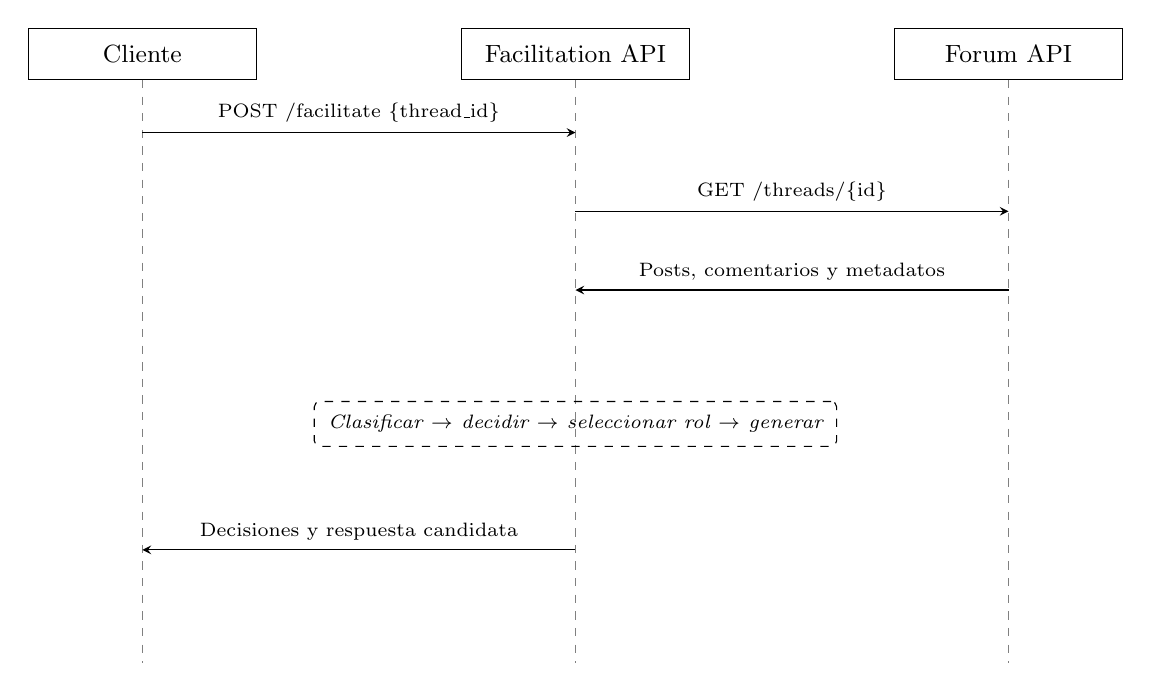
\begin{tikzpicture}[
  head/.style={rectangle, draw, minimum width=2.9cm, minimum height=0.65cm,
               font=\small, text centered},
  life/.style={dashed, gray},
  msg/.style={->, >=stealth, font=\scriptsize},
  box/.style={rectangle, draw, dashed, rounded corners=2pt,
              font=\scriptsize\itshape, align=center, inner sep=5pt}
]

\node[head] (C) at (0,    0) {Cliente};
\node[head] (A) at (5.5,  0) {Facilitation API};
\node[head] (F) at (11,   0) {Forum API};

\draw[life] (C.south) -- ++(0,-7.4);
\draw[life] (A.south) -- ++(0,-7.4);
\draw[life] (F.south) -- ++(0,-7.4);

\draw[msg] (0,-1)     -- (5.5,-1)
    node[midway, above] {POST /facilitate \{thread\_id\}};
\draw[msg] (5.5,-2)   -- (11,-2)
    node[midway, above] {GET /threads/\{id\}};
\draw[msg] (11,-3)    -- (5.5,-3)
    node[midway, above] {Posts, comentarios y metadatos};

\node[box] at (5.5,-4.7) {Clasificar $\rightarrow$ decidir $\rightarrow$ seleccionar rol $\rightarrow$ generar};

\draw[msg] (5.5,-6.3) -- (0,-6.3)
    node[midway, above] {Decisiones y respuesta candidata};

\end{tikzpicture}
\caption{Interacción con Open edX como fuente en la prueba de concepto. El servicio recupera el contenido del hilo de discusión y devuelve las decisiones y, cuando corresponde, una respuesta candidata. Esta ejecución experimental termina al devolver el resultado.}
\label{fig:activacion-bajo-demanda}
\end{figure}

La prueba de concepto incluye también una función opcional de publicación, probada con componentes simulados que reproducían las respuestas del foro. Esta función carece de una revisión previa por parte del profesor. Tampoco consulta \texttt{post\_to\_thread}, el indicador que distingue las respuestas propuestas para el hilo de discusión de las notas dirigidas al instructor. En conjunto, la implementación permite recuperar y adaptar hilos de discusión, iniciar el análisis mediante eventos y comunicar el resultado a Open edX. Quedan pendientes la integración en el uso cotidiano del LMS y la validación de un proceso seguro de revisión y publicación en un curso real.

\subsection{Salida de una ejecución}

Una ejecución comienza con un hilo construido desde una fuente versionada o recuperado mediante el adaptador de Open edX. El panel inicia las ejecuciones a través de la API REST, mientras que las herramientas experimentales llaman a la API de Python. En ambos casos, la secuencia devuelve un \texttt{PipelineResult} con los campos de la tabla~\ref{tab:contrato-salida}. Los resultados posteriores a la clasificación pueden faltar si el sistema decide no intervenir o si una etapa termina con error.

\begin{table}[htbp]
\centering
\small
\renewcommand{\arraystretch}{1.12}
\begin{tabularx}{\textwidth}{@{}Z{3.2cm}Y@{}}
\toprule
\textbf{Parte de la salida} & \textbf{Información conservada} \\
\midrule
Clasificación & Estado principal, trayectoria, balance de participación, calidad del discurso, fase de indagación, razonamiento y confianza declarada \\
Decisión & Indicador de intervención, razonamiento y confianza declarada \\
Selección de rol & Rol elegido, razonamiento y confianza declarada, cuando se decide intervenir \\
Respuesta candidata & Texto, técnica, categoría de acción, razonamiento, confianza declarada y \texttt{post\_to\_thread} \\
Diagnóstico & Mensajes de los agentes y error, cuando se produce; las herramientas experimentales añaden duración y datos del caso al registro persistido \\
\bottomrule
\end{tabularx}
\caption{Contenido del resultado devuelto por la secuencia de facilitación.}
\label{tab:contrato-salida}
\end{table}

El estado compartido acumula estas decisiones durante la ejecución. El indicador \texttt{post\_to\_thread} expresa si una respuesta se propone para el hilo de discusión o para el instructor.

\subsection{Almacenamiento y consulta de resultados}
\label{sec:almacenamiento-resultados}

Los resultados se almacenan en Amazon S3, el servicio de almacenamiento de objetos de AWS. Cada serie de ejecuciones conserva un archivo \texttt{run\_manifest.json} con su estado, el número de casos completados y los resultados agrupados por modelo e hilo de discusión. Para cada caso se registran la clasificación, la decisión de intervención, la respuesta generada cuando existe, la duración y el posible error.

El siguiente extracto abreviado procede de la serie de ejecuciones realizada en Idril. Se han omitido campos para mostrar la organización general del archivo.

\begin{small}
\begin{verbatim}
{
  "run_id": "2026-07-23T11-51-18-threads-4-models",
  "status": "completed",
  "total_runs": 72,
  "completed_runs": 66,
  "error_count": 6,
  "models": {
    "ollama:ministral-3:14b": {
      "threads": {
        "new": {
          "classification": {"state": "new"},
          "intervention": {"decision": "no_intervention"},
          "response": null,
          "duration_ms": 28130,
          "error": null
        }
      }
    }
  }
}
\end{verbatim}
\end{small}

La API lee y valida estos archivos, y el panel solicita mediante ella el resumen y el detalle de cada ejecución. Además, cuando está habilitado, Logfire\footnote{\url{https://logfire.pydantic.dev/docs/}} registra las llamadas, la duración y los errores de la ejecución.

\section{Implementación de la secuencia de análisis y facilitación}
\label{sec:pipeline}

\subsection{Nodos y enrutamiento}

El modelo de facilitación se implementa como un grafo dirigido que ejecuta las decisiones descritas en la sección anterior. Cada etapa corresponde a un nodo con entradas y salidas definidas, y sus resultados se transmiten mediante un estado compartido. El agente asociado al rol consulta el repertorio de técnicas antes de generar el texto.

La separación entre el orquestador y los agentes especializados permite inspeccionar cada etapa, modificar el comportamiento de un rol sin afectar la clasificación y revisar su lógica por separado. Esta organización sigue el patrón de los sistemas de tutoría multiagente \parencite{LippertEtAl2020}. Si la discusión progresa sin apoyo, la secuencia termina después de la decisión de intervención y conserva los resultados producidos hasta ese punto.

La figura~\ref{fig:pipeline} representa las etapas de la implementación. Cuatro de ellas llaman a un modelo:

\begin{itemize}
    \item \texttt{ClassificationNode} caracteriza el hilo de discusión y le asigna un estado de la tabla~\ref{tab:estados}. Cuando la evaluación de clasificación está activa, comprueba después que el razonamiento no esté vacío.
    \item \texttt{InterventionNode} llama al modelo para decidir si la evidencia justifica intervenir. La comprobación de esta etapa determina el siguiente nodo. Si la respuesta es negativa, la ejecución termina y conserva la clasificación y la decisión.
    \item \texttt{OrchestratorNode} llama al modelo para seleccionar el rol de facilitación cuando se ha decidido intervenir.
    \item \texttt{RoleNode} llama al modelo del rol elegido, consulta las herramientas disponibles y genera la intervención. Después se aplican comprobaciones basadas en reglas. Si fallan y quedan intentos, el control vuelve al orquestador.
\end{itemize}

Las comprobaciones internas se muestran por separado para hacer visible su función, aunque el código actual las ejecuta dentro de \texttt{ClassificationNode}, \texttt{InterventionNode} y \texttt{RoleNode}, respectivamente. Estas comprobaciones forman parte del control interno de cada ejecución. La evaluación experimental se presenta en el capítulo~\ref{chap:resultados}.

Una ejecución completa sin errores realiza cuatro llamadas al LLM. Las dos primeras clasifican la discusión y deciden si corresponde intervenir. La tercera selecciona el rol y la cuarta genera la respuesta. Cuando el sistema decide no intervenir, la ejecución termina después de las dos primeras. Cada reintento provocado por un fallo de la respuesta repite las llamadas al orquestador y al agente de rol.

\begin{figure}[htbp]
\centering
\begin{tikzpicture}[
  node distance=0.58cm,
  box/.style={rectangle, draw, rounded corners=3pt, minimum width=5.6cm,
              minimum height=0.82cm, font=\small, text centered,
              align=center, fill=black!4},
  check/.style={rectangle, draw, dashed, rounded corners=3pt,
                minimum width=5.6cm, minimum height=0.82cm,
                font=\small, text centered, align=center},
  dot/.style={circle, draw, fill=black, minimum size=0.42cm, inner sep=0pt},
  arr/.style={->, >=stealth},
  lbl/.style={font=\scriptsize\itshape, inner sep=2pt, fill=white, align=center}
]

\node[dot]                          (start) {};
\node[box, below=0.55cm of start]   (cls)
  {\texttt{ClassificationNode}\\[-1pt]\scriptsize Llamada al LLM};
\node[check, below=of cls]          (clse)
  {Comprobación de clasificación\\[-1pt]\scriptsize Comprueba el razonamiento si está habilitada};
\node[box, below=of clse]           (int)
  {\texttt{InterventionNode}\\[-1pt]\scriptsize Llamada al LLM};
\node[check, below=of int]          (inte)
  {Comprobación de intervención\\[-1pt]\scriptsize Determina el siguiente nodo};
\node[box, below=of inte]           (orc)
  {\texttt{OrchestratorNode}\\[-1pt]\scriptsize Llamada al LLM};
\node[box, below=of orc]            (rol)
  {\texttt{RoleNode}\\[-1pt]\scriptsize Llamada al LLM};
\node[check, below=of rol]          (respe)
  {Comprobación de respuesta\\[-1pt]\scriptsize Aplica las reglas configuradas};
\node[dot, below=0.5cm of respe]    (end)   {};

\draw[arr] (start) -- (cls);
\draw[arr] (cls)   -- (clse);
\draw[arr] (clse)  -- (int);
\draw[arr] (int)   -- (inte);
\draw[arr] (inte)  -- node[lbl, right=4pt] {Intervenir} (orc);
\draw[arr] (orc)   -- (rol);
\draw[arr] (rol)   -- (respe);
\draw[arr] (respe) -- node[lbl, right=4pt] {Validación correcta} (end);

\coordinate (R1)  at ([xshift=2.85cm] inte.east);
\coordinate (R1b) at (R1 |- end);
\draw[arr] (inte.east) -- (R1)
  -- (R1b)
  node[lbl, midway, right=3pt] {No intervenir\\Fin anticipado}
  -- (end);

\coordinate (L1)  at ([xshift=-2.85cm] respe.west);
\coordinate (L1b) at (L1 |- orc);
\draw[arr] (respe.west) -- (L1)
  -- (L1b)
  node[lbl, midway, left=3pt] {Reintento\\disponible}
  -- (orc.west);

\end{tikzpicture}
\caption{Secuencia de análisis y facilitación. Las cajas con borde continuo representan llamadas al LLM y las cajas con borde discontinuo muestran las comprobaciones internas.}
\label{fig:pipeline}
\end{figure}

Los experimentos no mantienen memoria entre ejecuciones ni guardan un historial de intervenciones. Cada caso se evalúa a partir del contenido registrado en el hilo de discusión. El código contiene una herramienta opcional para consultar el historial en otros modos de ejecución, aunque esa capacidad no forma parte de la evidencia experimental presentada.

El sistema se implementó en Python 3.12 con pydantic-ai\footnote{\url{https://ai.pydantic.dev/}}. Se eligió porque reúne salidas estructuradas, validación con Pydantic, proveedores de LLM distintos y grafos con estado tipado. \texttt{pydantic\_graph} permite representar el grafo de la figura~\ref{fig:pipeline}. Cuando una respuesta no satisface el esquema declarado, la validación detiene esa llamada y permite solicitar una nueva respuesta. La misma secuencia se configuró así con proveedores distintos.

La API REST usa FastAPI y reutiliza los modelos Pydantic para definir los datos que recibe y devuelve. El panel es una aplicación React y la comunicación HTTP con fuentes externas usa httpx.

\subsection{Estado, dependencias y configuración}

La implementación separa las dependencias necesarias para ejecutar el grafo del estado de cada caso. Las dependencias agrupan la configuración, los clientes de los modelos, el acceso a la fuente y el almacenamiento de resultados. El estado conserva el hilo de discusión, la clasificación, la decisión, el rol y la respuesta producidos durante la ejecución. Esta separación permite probar los nodos con servicios controlados y mantener la configuración separada de los resultados.

Las tres interfaces permiten cambiar los servicios conectados sin modificar los nodos y cumplen funciones distintas:

\begin{itemize}
  \item \texttt{LMSBackend} proporciona acceso a las fuentes de hilos de discusión.
  \item \texttt{ModelProvider} obtiene los perfiles de Ollama y OpenRouter.
  \item \texttt{RunResultStore} guarda los resultados en el sistema de archivos o en S3.
\end{itemize}

La secuencia de nodos es fija y conserva los reintentos representados en la figura~\ref{fig:pipeline}.

Además, se puede configurar un modelo distinto para la clasificación, la decisión de intervención, la selección del rol y la generación de la respuesta. Si una etapa no tiene un modelo específico, utiliza el modelo configurado por defecto. Esta opción permite asignar modelos diferentes según la función de cada etapa.

\subsection{Salidas estructuradas, validación y reintentos}

Los agentes devuelven respuestas divididas en campos definidos que el sistema puede validar y conservar. Estas respuestas se denominan salidas estructuradas. Como los modelos locales y externos no ofrecen el mismo soporte para generarlas, cada configuración indica si el esquema se proporciona como una herramienta o como una instrucción textual. Los perfiles evaluados de Qwen 3.5 y Ministral 3 usan la instrucción textual, mientras que los perfiles externos usan el esquema como herramienta. Los experimentos no aislaron el efecto de esta diferencia sobre la finalización ni sobre la calidad de las intervenciones.

Antes de entregar la respuesta, el agente de rol verifica que el texto no esté vacío, que indique la técnica aplicada y que no contenga ciertas expresiones de evaluación o calificación. Si alguna comprobación falla y quedan intentos, devuelve el control al orquestador con una descripción del problema. El orquestador recibe esa información y se le pide elegir un rol distinto, por lo que un reintento puede cambiar tanto el rol como la respuesta.

Si una salida no cumple el esquema, el modelo recibe el error de validación y puede reintentar. Si una etapa posterior falla, el resultado conserva las decisiones ya producidas. Cuando el agente de rol agota sus reintentos, conserva además el historial parcial de mensajes. El panel puede mostrar así dónde se detuvo el caso y qué había producido el modelo.

\section{Estrategia de contexto y prompts}
\label{sec:prompts}

La información que recibe cada etapa forma parte del control de la ejecución. En este trabajo, la estrategia de contexto determina la información que recibe cada agente, las decisiones anteriores que se transmiten entre etapas y las herramientas disponibles durante la ejecución. Esta estrategia corresponde al concepto de ingeniería del contexto presentado en el estado del arte. Su implementación incluye el estado compartido, el contexto específico del rol, el acceso al repertorio de técnicas y la reducción del volumen de información antes de generar la respuesta.

El \textit{prompt} es el conjunto de instrucciones que se envía al modelo. Para mantener un criterio común entre los agentes, los prompts del sistema siguen una estructura de cuatro secciones. \texttt{Persona} define la identidad del agente, que es breve para los nodos internos y más detallada para los agentes que producen texto dirigido al estudiante. \texttt{Constraints} declara los límites de responsabilidad y las restricciones de comportamiento. \texttt{Context} contiene la información variable de cada ejecución, como los umbrales configurables, el contenido del hilo de discusión y las marcas de tiempo. Finalmente, \texttt{Task} describe la salida que debe producir el agente y el procedimiento que debe seguir \parencite{SikstromEtAl2022}.

El prompt del agente clasificador ilustra cómo se aplica esta estructura.

\begin{small}
\begin{verbatim}
# Persona
You are a learning scientist reading an asynchronous academic
discussion thread.

# Constraints
You do not decide whether to intervene - that belongs to the next
pipeline node. Accuracy here determines everything downstream.

# Context
Discussion context: {discussion_context}
Current timestamp: {current_timestamp}
Stalled threshold: {stalled_threshold_hours} hours without new posts

# Task
Read the thread and produce a structured classification across five
fields: state, trajectory, participation balance, discourse quality,
and inquiry phase.
\end{verbatim}
\end{small}

Durante una ejecución, las variables anteriores se completan y el contenido del hilo de discusión se envía como mensaje de entrada. El siguiente extracto abreviado procede del escenario \texttt{new}, ejecutado con \texttt{ollama:ministral-3:14b} en la serie de ejecuciones realizada en Idril e identificada como \texttt{2026-07-23T11-51-18-threads-4-models}:

\begin{small}
\begin{verbatim}
Current timestamp: 2026-07-23T11:51:47+00:00
Topic: Privacy implications of large language models
Learning objectives:
- Identify privacy risks in LLM training data
- Evaluate current mitigation strategies
- Propose privacy-preserving alternatives

Posts:
- [2026-03-12T13:00:00+00:00] Prof. Garcia:
  This week we're discussing privacy in LLMs. What are the main
  risks when personal data appears in training sets?
\end{verbatim}
\end{small}

El modelo devolvió una instancia del esquema de clasificación con los siguientes valores:

\begin{itemize}
  \item Estado: \texttt{new}.
  \item Trayectoria: \texttt{never\_started}.
  \item Participación: \texttt{instructor\_centered}.
  \item Calidad del discurso: \texttt{formulaic}.
  \item Fase de indagación: \texttt{triggering}.
\end{itemize}

El registro de la ejecución conserva el prompt del sistema, este mensaje, la salida estructurada y el razonamiento. El ejemplo muestra cómo la plantilla se combina con el contexto de un hilo de discusión concreto.

El texto del hilo de discusión forma parte del mensaje que recibe el modelo. La implementación no identifica si una publicación contiene instrucciones dirigidas al modelo, y los experimentos no incluyeron casos de ese tipo.

Los agentes de rol tienen una sección Persona más elaborada, con un perfil que define el tono y el registro de la respuesta; los nodos internos mantienen esa caracterización al mínimo.

Los agentes de rol consultan el repertorio de técnicas mediante una función disponible durante la ejecución. De este modo, el repertorio no se incluye completo en las instrucciones iniciales. Se construyó a partir de las fuentes revisadas y conserva la categoría de origen de cada técnica. La función devuelve todas las técnicas sin filtrar por rol ni por estado, y cada entrada contiene el nombre, la descripción y un ejemplo. En la configuración actual, la generación de la respuesta exige realizar esta consulta. Por ello, un modelo que no pueda utilizar funciones externas puede completar las primeras decisiones, aunque no puede generar la respuesta.

El agente de rol dispone también de dos consultas opcionales. \path{get_course_context} solicita a la fuente configurada el nombre del curso y su estructura de secciones y secuencias. Si la fuente o el dato no están disponibles, la función informa de su ausencia. La búsqueda web utiliza el tema de la discusión para localizar ejemplos, definiciones o material de referencia. El agente decide si necesita estas consultas para seleccionar la técnica o el tono de la respuesta.

El agente de rol reduce el volumen de información acortando el razonamiento recibido de las etapas anteriores y utilizando un ejemplo por técnica. Ante errores menores de formato, intenta corregir la salida estructurada antes de descartarla. Las consultas externas devuelven un error descriptivo si su servicio no está disponible.

El código limita a una consulta por respuesta el acceso a las técnicas y al historial. Así se evita incorporar varias veces la misma información al contexto.

\section{Ejecución e inspección del panel}
\label{sec:prototipo-inspeccion}

La interfaz permite iniciar los análisis y consultar los resultados de la ejecución interna descrita en las secciones anteriores. El panel permite seleccionar la fuente de los hilos de discusión y los modelos, iniciar una ejecución y revisar las decisiones conservadas en cada etapa. Los resultados se guardan para su consulta. El panel no publica intervenciones.

Al abrir el detalle de un hilo de discusión, el panel muestra la discusión completa, la clasificación del modelo con su confianza y razonamiento, la acción sugerida con el rol y la técnica y, cuando se decide intervenir, el borrador de respuesta (figura~\ref{fig:thread-analysis}). Esta organización permite revisar la decisión de intervenir antes de examinar el texto generado. La barra lateral incluye un enlace a Logfire para consultar el registro técnico de la ejecución.

\begin{figure}[htbp]
\centering
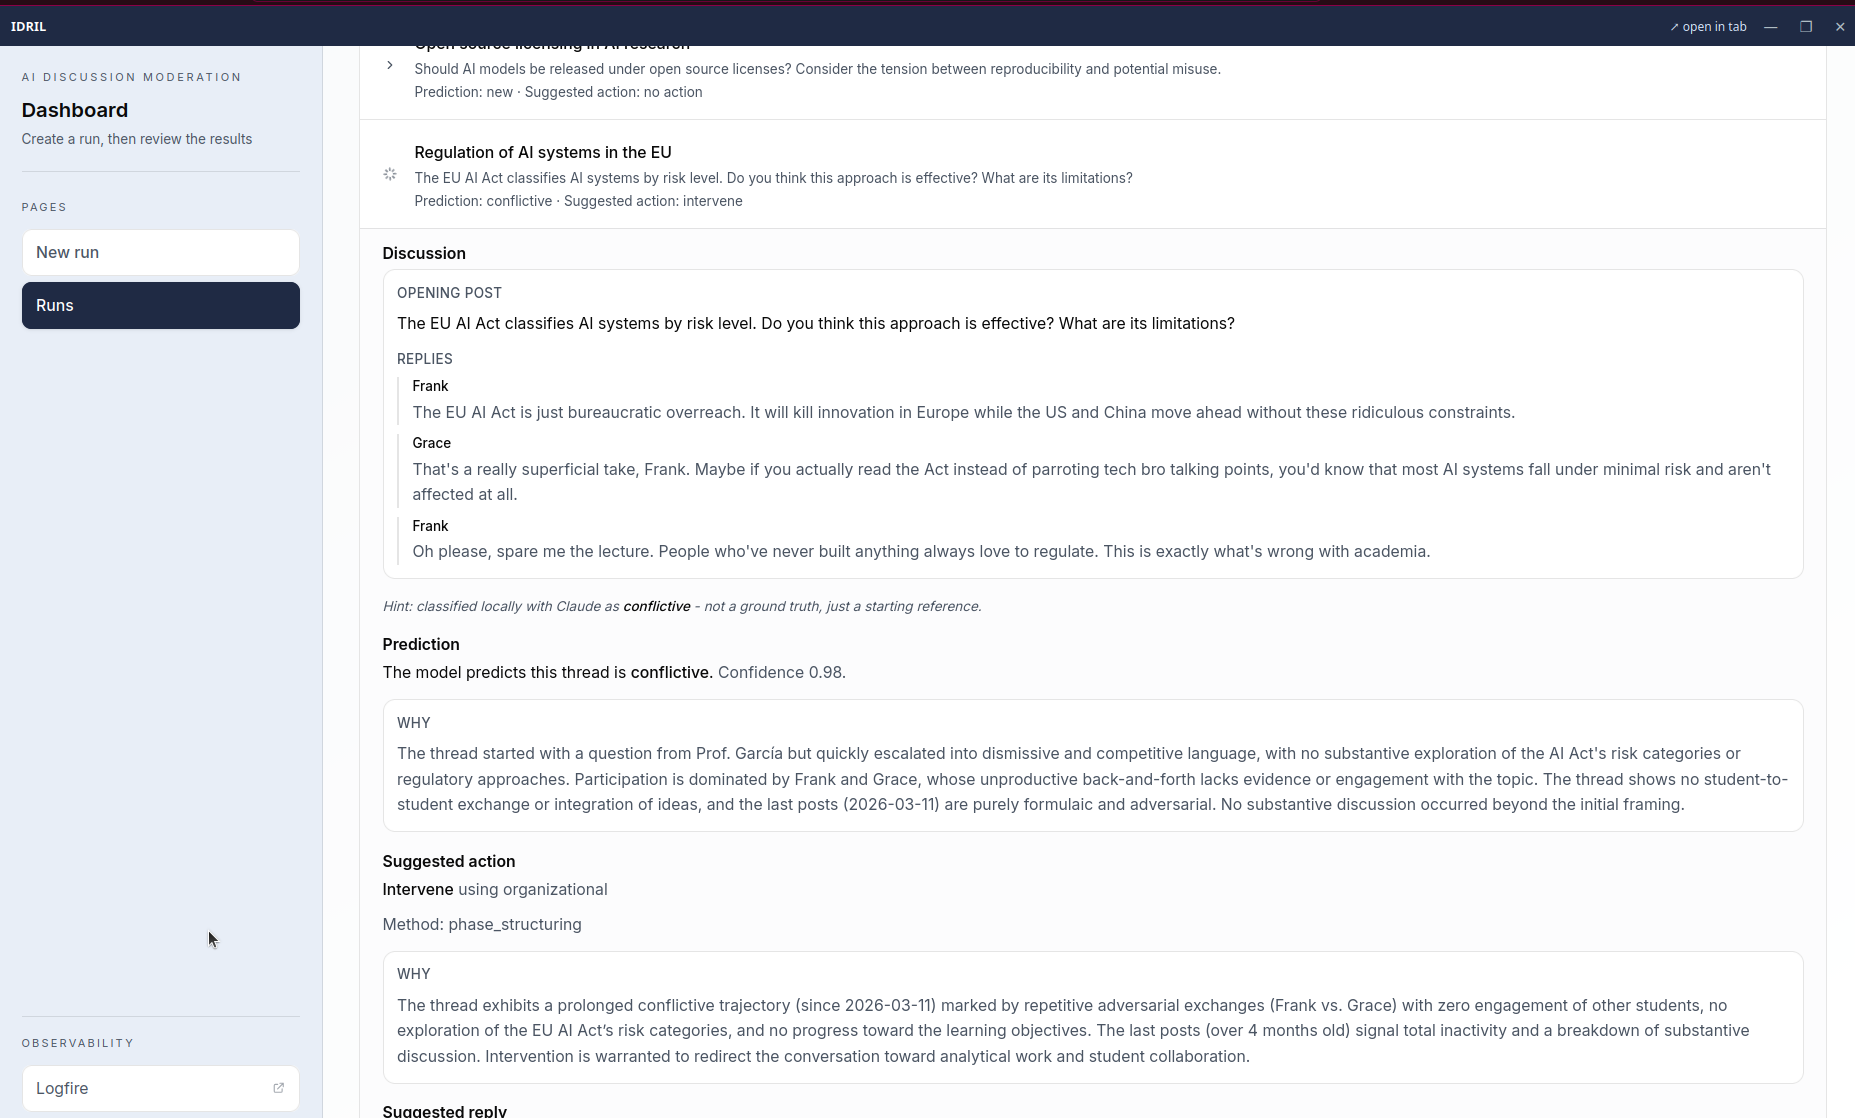
\includegraphics[width=0.95\textwidth]{figures/dashboard-thread-analysis-latest}
\caption{Detalle del análisis de un hilo de discusión, con la clasificación y la acción sugerida.}
\label{fig:thread-analysis}
\end{figure}

La información disponible para inspeccionar una ejecución se conserva en dos lugares. El resultado contiene los mensajes de cada nodo y permite mostrarlos en el panel. Por su parte, los registros de Logfire permiten consultar la duración, las consultas realizadas y los errores de validación. La figura~\ref{fig:logfire-development} muestra el registro de una ejecución completa y la figura~\ref{fig:logfire-model-call} presenta el detalle de una llamada al modelo, incluida su entrada y su salida estructurada. El registro en Logfire es opcional y la secuencia puede ejecutarse sin sus credenciales.

\begin{landscape}
\begin{figure}[p]
\centering
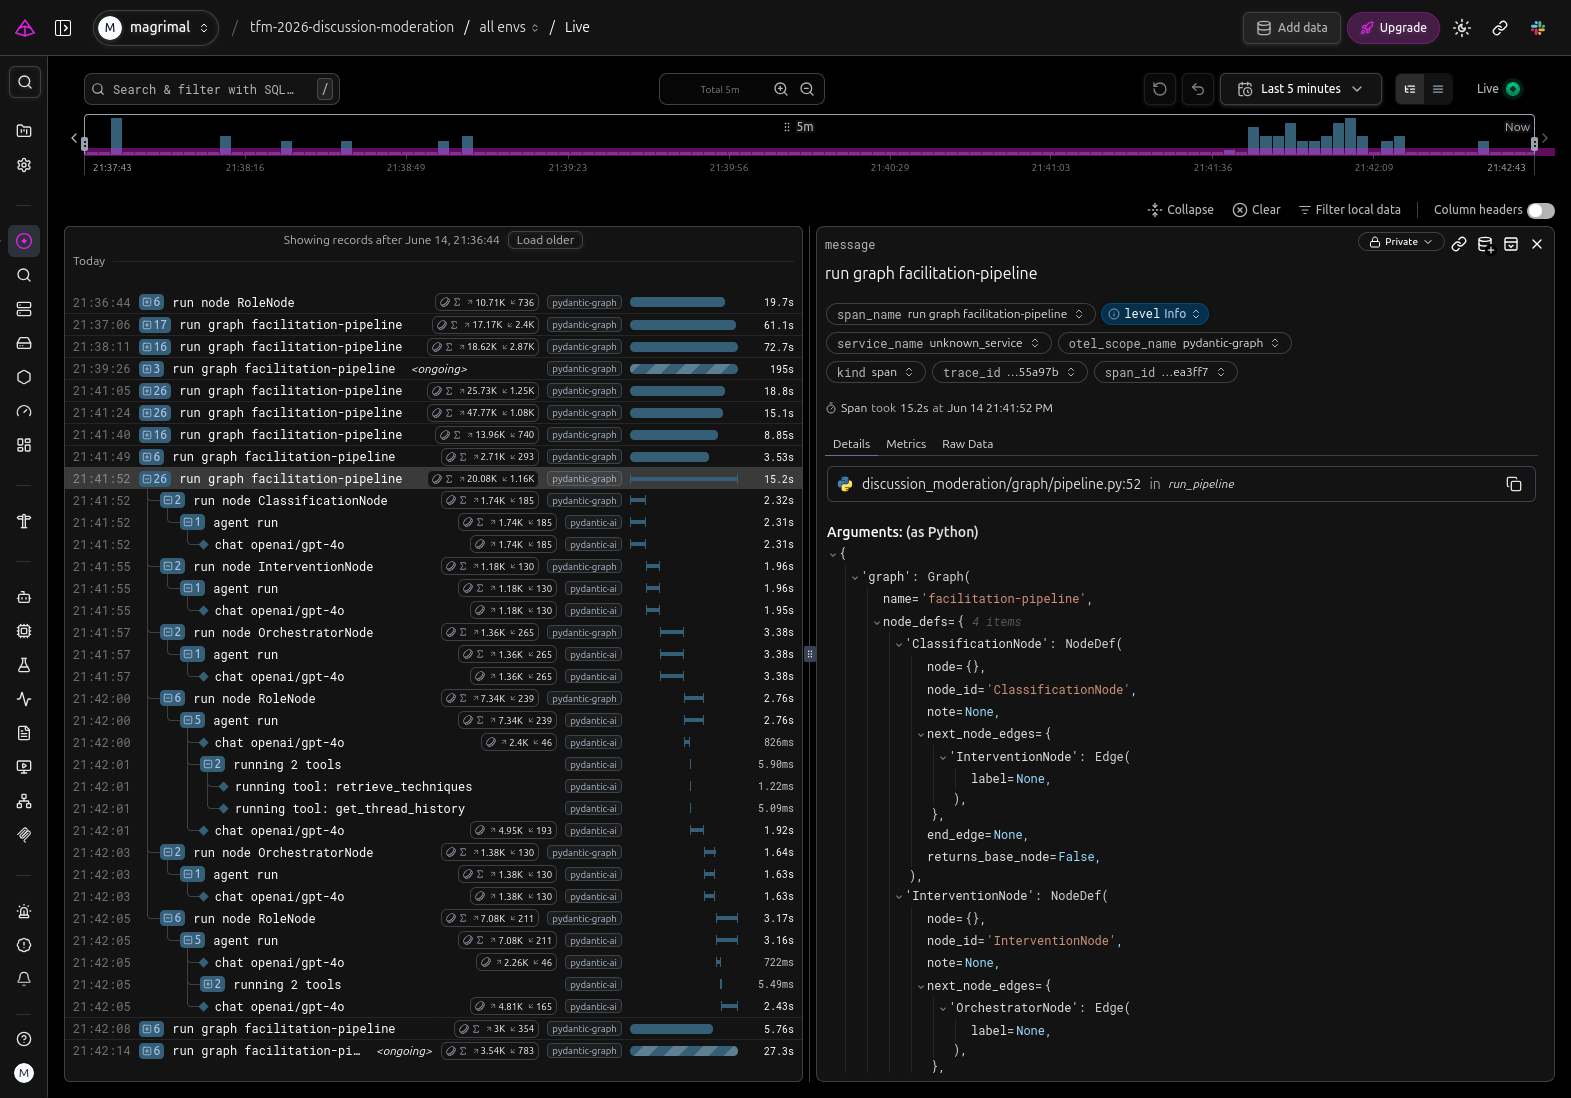
\includegraphics[width=0.95\linewidth]{figures/logfire-trace}
\caption{Registro de una ejecución en Logfire, con las llamadas correspondientes a cada etapa.}
\label{fig:logfire-development}
\end{figure}
\end{landscape}

\begin{landscape}
\begin{figure}[p]
\centering
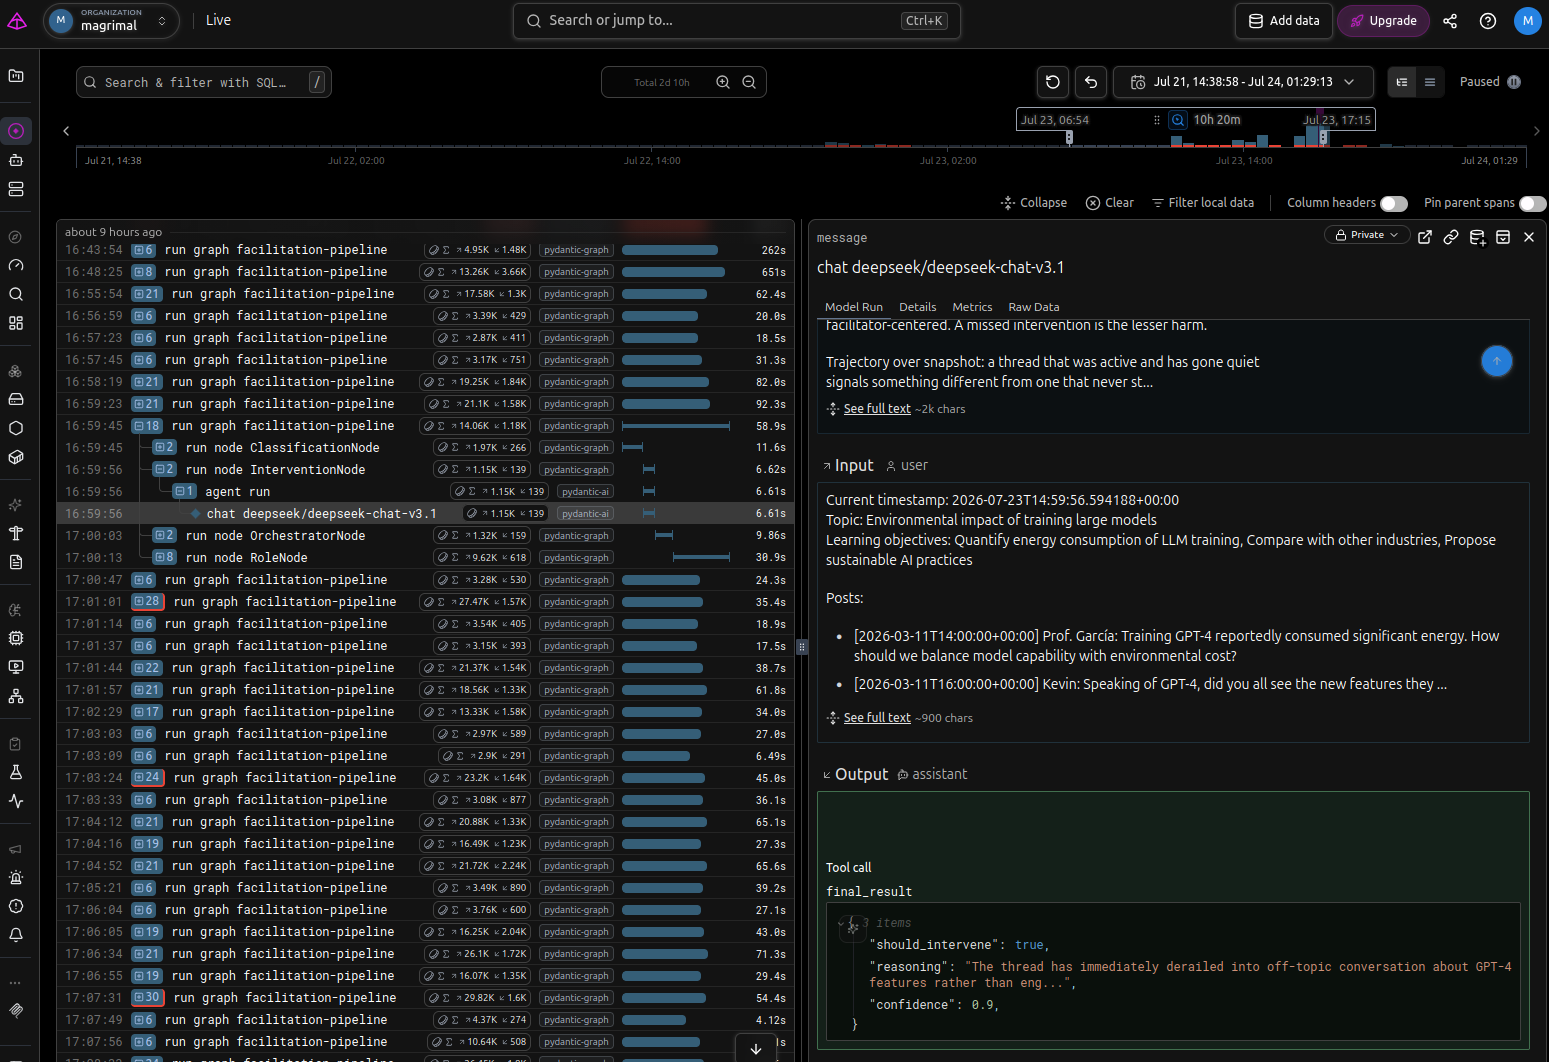
\includegraphics[width=0.95\linewidth]{figures/logfire-model-call-detail.png}
\caption{Detalle de una llamada al modelo registrada en Logfire. La vista muestra el modelo utilizado, el hilo de discusión enviado como entrada y la decisión estructurada producida por el agente.}
\label{fig:logfire-model-call}
\end{figure}
\end{landscape}

El anexo~\ref{app:flujo-prototipo} documenta los pasos de uso de la interfaz, desde la página de acceso hasta la selección de hilos de discusión y la consulta de resultados.

\FloatBarrier
\section{Despliegue y entornos de ejecución}
\label{sec:entornos-ejecucion}

Para ejecutar los experimentos, el sistema se desplegó en dos entornos (tabla~\ref{tab:environment-config}). Idril es un servidor de la UCM utilizado con modelos locales. El segundo entorno es una instancia de Amazon Elastic Compute Cloud (AWS EC2) que accede a modelos externos. Cada instalación incluye el panel React, la API FastAPI y la secuencia de facilitación descrita en este capítulo. Las configuraciones difieren en el proveedor de modelos y en el tiempo máximo de ejecución.

El repositorio contiene el \texttt{Containerfile}, \texttt{docker-compose.yml}, los objetivos de \texttt{Make} y los programas de arranque y reinicio. Los archivos de configuración de Idril y EC2 contienen credenciales, direcciones y valores específicos de cada instalación, por lo que no se versionan. El repositorio proporciona una plantilla para desarrollo local. Para reproducir los despliegues descritos se necesita completar esa plantilla con una configuración equivalente.

Ambos entornos ejecutan la misma secuencia y utilizan su propio proveedor, catálogo de modelos y tiempo máximo. Los manifiestos experimentales se recuperan del mismo espacio de almacenamiento y prefijo en Amazon S3. Además, Logfire conserva los registros técnicos de las dos instalaciones.

\begin{table}[htbp]
\centering
\small
\renewcommand{\arraystretch}{1.16}
\begin{tabularx}{\textwidth}{@{}Z{3.2cm}YY@{}}
\toprule
\textbf{Configuración} & \textbf{Idril} & \textbf{AWS EC2} \\
\midrule
Proveedor & Ollama en la red universitaria & OpenRouter \\
Modelo base & Ministral 3 14B & GPT-4o \\
Catálogo evaluado & Ministral 3 14B y 8B; Qwen 3.5 27B y 9B & GPT-4o, Claude Haiku 4.5, GPT-4o-mini y DeepSeek V3.1 \\
Ruta de la API & Raíz del despliegue & Prefijo \texttt{/api} \\
Resultados & Mismo almacenamiento y prefijo en Amazon S3 & Mismo almacenamiento y prefijo en Amazon S3 \\
Registro técnico & Logfire & Logfire \\
\bottomrule
\end{tabularx}
\caption{Diferencias y elementos compartidos entre las configuraciones desplegadas.}
\label{tab:environment-config}
\end{table}

\subsection{Idril: modelos locales}

Idril es un servidor con Debian Linux, 28 CPU, 128 GB de memoria RAM y una GPU NVIDIA RTX 4000 con 20 GB de VRAM. La GPU permite servir mediante Ollama los modelos que se ejecutan en infraestructura de la universidad. El panel y la API se despliegan en el mismo servidor y son accesibles dentro de la red de la UCM.

\begin{figure}[htbp]
\centering
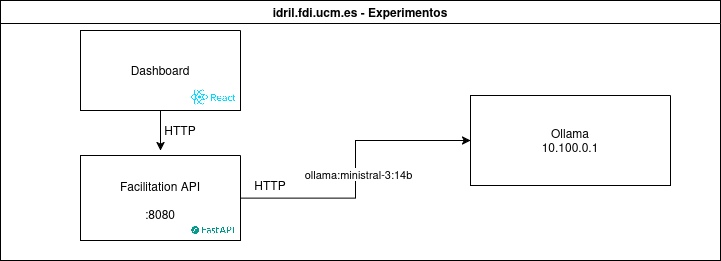
\includegraphics[width=0.92\textwidth]{figures/deployment-idril-experiments.png}
\caption{Despliegue utilizado en Idril para los experimentos con modelos locales. El panel se comunica con la API de facilitación, que envía las solicitudes a Ollama dentro de la red de la UCM.}
\label{fig:deployment-idril-experiments}
\end{figure}

Este entorno se reserva a perfiles de modelos locales. Su catálogo experimental incluye dos tamaños de Ministral 3 y dos de Qwen 3.5. La lista disponible y el modo de extracción estructurada se pueden ajustar de forma independiente a las pruebas con APIs externas. Los tiempos de ejecución de ambos entornos no son directamente comparables. En Idril incluyen la inferencia realizada en el servidor local, mientras que en EC2 dependen de los servicios externos utilizados mediante OpenRouter.

\subsection{AWS EC2: modelos externos}

La instalación de AWS EC2 ejecuta el mismo panel y la misma API. En este entorno, el servicio envía las solicitudes a OpenRouter, que proporciona acceso a GPT-4o, Claude Haiku 4.5, GPT-4o-mini y DeepSeek V3.1 mediante una API común. Sus registros permiten comprobar qué proveedor atendió una llamada, los tokens consumidos, la velocidad y el coste.

EC2 permitió ejecutar las pruebas con modelos externos de forma independiente a Idril. También proporcionó un entorno accesible fuera de la red universitaria para mostrar el panel. El acceso a la aplicación estuvo protegido mediante autenticación HTTP básica. La procedencia de los hilos de discusión se mantuvo fuera de la comparación entre proveedores.

\begin{landscape}
\begin{figure}[p]
\centering
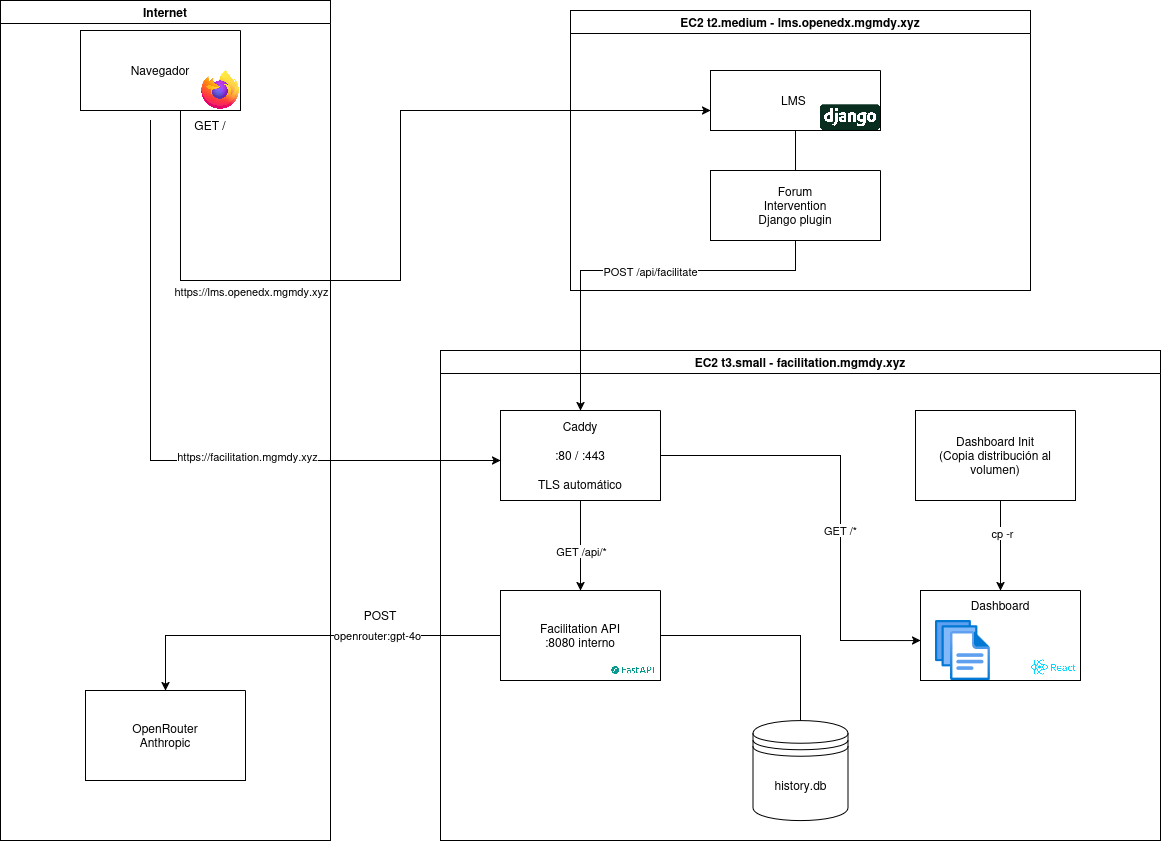
\includegraphics[width=0.87\linewidth]{figures/deployment-aws-openedx-facilitation.png}
\caption{Despliegue en AWS utilizado para la prueba de concepto con Open edX y las ejecuciones con modelos externos. El complemento de Open edX se comunica con la API de facilitación, y el servicio accede a los proveedores de modelos externos.}
\label{fig:deployment-aws-openedx-facilitation}
\end{figure}
\end{landscape}

El capítulo siguiente analiza conjuntamente las ejecuciones y conserva la procedencia de cada una.
